%You can leave alone everything before Line 79.
\documentclass{article}
\usepackage{url,amsfonts, amsmath, amssymb, amsthm,color, enumerate, verbatim}
% Page layout
\setlength{\textheight}{8.75in}
\setlength{\columnsep}{2.0pc}
\setlength{\textwidth}{6.5in}
\setlength{\topmargin}{0in}
\setlength{\headheight}{0.0in}
\setlength{\headsep}{0.0in}
\setlength{\oddsidemargin}{0in}
\setlength{\evensidemargin}{0in}
\setlength{\parindent}{1pc}
\newcommand{\shortbar}{\begin{center}\rule{5ex}{0.1pt}\end{center}}
%\renewcommand{\baselinestretch}{1.1}
% Macros for course info
\newcommand{\courseNumber}{ME 552}
\newcommand{\courseTitle}{Mechatronics}
\newcommand{\semester}{Fall 2012}
\newcommand{\xxx}[1]{\textcolor{red}{#1}}
% Theorem-like structures are numbered within SECTION units
\theoremstyle{plain}
\newtheorem{theorem}{Theorem}[section]
\newtheorem{lemma}[theorem]{Lemma}
\newtheorem{corollary}[theorem]{Corollary}
\newtheorem{proposition}[theorem]{Proposition}
\newtheorem{statement}[theorem]{Statement}
\newtheorem{conjecture}[theorem]{Conjecture}
\newtheorem{fact}{Fact}
%definition style
\theoremstyle{definition}
\newtheorem{definition}[theorem]{Definition}
\newtheorem{example}{Example}
\newtheorem{problem}[theorem]{Problem}
\newtheorem{exercise}{Exercise}
\newtheorem{algorithm}{Algorithm}
%remark style
\theoremstyle{remark}
\newtheorem{remark}[theorem]{Remark}
\newtheorem{reduction}[theorem]{Reduction}
%\newtheorem{question}[theorem]{Question}
\newtheorem{question}{Question}
%\newtheorem{claim}[theorem]{Claim}
%
% Proof-making commands and environments
\newcommand{\beginproof}{\medskip\noindent{\bf Proof.~}}
\newcommand{\beginproofof}[1]{\medskip\noindent{\bf Proof of #1.~}}
\newcommand{\finishproof}{\hspace{0.2ex}\rule{1ex}{1ex}}
\def\therefore{\boldsymbol{\text{ }
\leavevmode
\lower0.4ex\hbox{$\cdot$}
\kern-.5em\raise0.7ex\hbox{$\cdot$}
\kern-0.55em\lower0.4ex\hbox{$\cdot$}
\thinspace\text{ }}}

\newenvironment{solution}[1]{\medskip\noindent{\bf Problem #1.~}}{\shortbar}

%====header======
\newcommand{\solutions}[4]{
%\renewcommand{\thetheorem}{{#2}.\arabic{theorem}}
\vspace{-2ex}
\begin{center}
{\small  \courseNumber, \courseTitle
\hfill {\Large \bf {#1} }\\
\semester, University of Michigan, Ann Arbor \hfill
{\em Date: #3}}\\
\vspace{-1ex}
\hrulefill\\
\vspace{4ex}
{\LARGE Lab Assignment #2}\\
\vspace{2ex}
\end{center}
\begin{trivlist}
\item \textsc{Team members:\\} {#4}
\end{trivlist}
\noindent
\shortbar
\vspace{3ex}
}
% math macros
\newcommand{\defeq}{\stackrel{\textrm{def}}{=}}
\newcommand{\Prob}{\textrm{Prob}}
\newcommand{\Lagr}{\mathcal{L}}
%==
\usepackage{graphicx}
\usepackage{xfrac}
\usepackage{amsmath}
\providecommand{\e}[1]{\ensuremath{\times 10^{#1}}}
\begin{document}
%%%%%%%%%%%%%%%%%%%%%%%%%%%%%%%%%%%%%%%%%%%%%%%%%
%\solutions{Your name}{Problem Set Number}{Date of preparation}{Collaborators}{Prover}{Verifiers}
\solutions{}{5: Stepper Motor}{\today}{Shiva Ghose, @gshiva\\ John Peterson, @jrpeters\\ Peter Turpel, @pturpel\\ Chan-Rong Lin, @pmelin}
%%%%%%%%%%%%%%%%%%%%%%%%%%%%%%%%%%%%%%%%%%%%%%%%%
%\renewcommand{\theproblem}{\arabic{problem}} 
%%%%%%%%%%%%%%%%%%%%%%%%%%%%%%%%%%%%%%%%%%%%%%%%%
%
% Begin the solution for each problem by
% \begin{solution}{Problem Number} and ends it with \end{solution}
%
% the solution for Problem 
\section*{Teamwork Participation Pledge :: Team 1}

I attest that I have made a fair and equitable contribution to this lab and submitted 
assignment. \\

My signature also indicates that I have followed the University of Michigan Honor Code, 
while working on this lab and assignment.\\

I accept my responsibility to look after all of the equipment assigned to me and my team, 
and that I have read and understood the X50 Lab Rules.\\

\begin{table}[h]
\begin{center}
    \begin{tabular}{|c|c|c|}
        \hline
        \textbf{Name} & \textbf{Email}     & \textbf{ \ \ \ \ \  \ \  \ \ \ \ \  \ \ Signature  \ \ \ \ \  \ \ \ \ \ \ \  \ \ } \\ \hline
        	~& ~& ~\\
	~& ~& ~\\
	Shiva Ghose   & gshiva@umich.edu   & ~                  \\
	~& ~& ~\\
	~& ~& ~\\ \hline 
	~& ~& ~\\
	~& ~& ~\\
        John Peterson & jrpeters@umich.edu & ~                  \\ 
	~& ~& ~\\
	~& ~& ~\\ \hline 
	~& ~& ~\\
	~& ~& ~\\
        Peter Turpel   & pturpel@umich.edu & ~                  \\
	~& ~& ~\\
	~& ~& ~\\ \hline 
	~& ~& ~\\
	~& ~& ~\\
        Chan-Rong Lin   & pmelin@umich.edu & ~                  \\
	~& ~& ~\\
	~& ~& ~\\ \hline 
        \hline
    \end{tabular}
\end{center}
\end{table}

\newpage

\section{Stepper Motor Driver}
\subsection*{a.}

\begin{figure}[htb]
\begin{center}
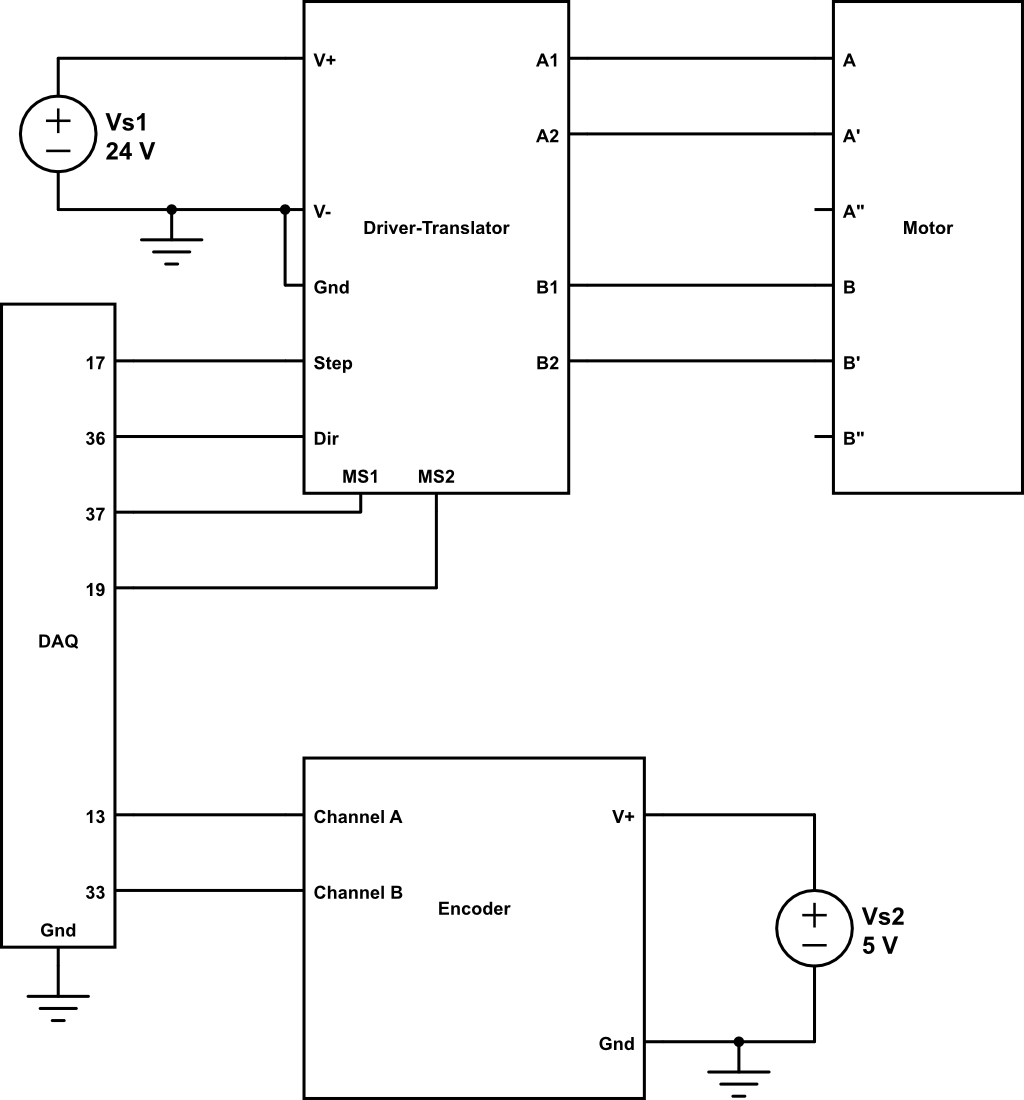
\includegraphics[width = 12cm]{lab5_main.png}
\caption{System level connection diagram. \xxx{Note all grounds are common}}
\label{q1_a}
\end{center}
\end{figure}

\subsection*{b.}
\begin{figure}[htb]
\begin{center}
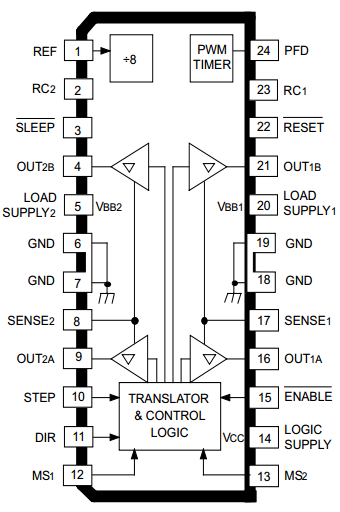
\includegraphics[width = 5cm]{A3967_pinout.png}
\caption{Pinout diagram of the A3967 chip.}
\label{q1_b}
\end{center}
\end{figure}

\begin{figure}[htb]
\begin{center}
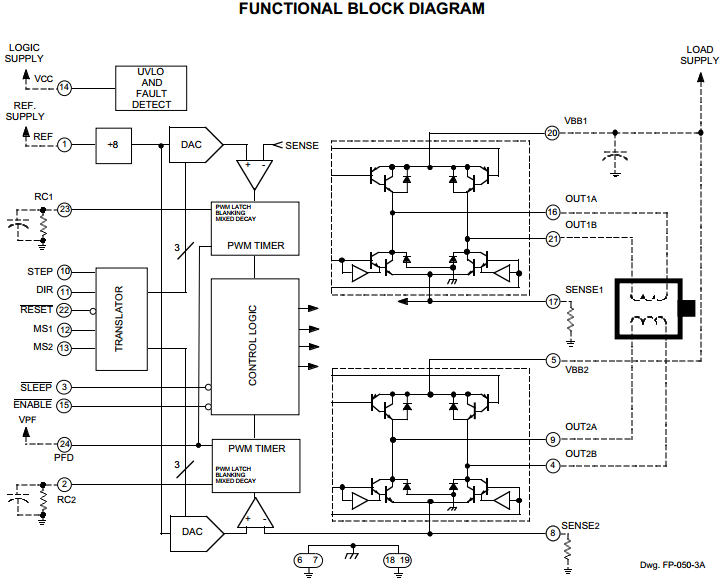
\includegraphics[width = 14cm]{A3967_functionalDiagram.png}
\caption{Functional diagram of the A3967 chip.}
\label{q1_b2}
\end{center}
\end{figure}

\subsubsection*{Pin1 - REF}
The \emph{REF} pin of the A3967 chip takes set the reference voltage for the logic circuit $V_{REF}$. It works with tandem with the senseristor to control the magnitude of the H-bridge current in the following manner:
\begin{itemize}
\item At $V_{REF} = 5$V max current will be 833mA.
\item At $V_{REF} = 3.3$V max current will be 550mA.
\item At $V_{REF} = 1$V max current will be 166mA.
\end{itemize}

From the functional diagram (figure \ref{q1_b2}), we see that $V_{REF}$ is fed into a DAC which is then fed to a comparator which then controls the PWM output, which in turn controls the current.\\

This input does not strictly require a dedicated external circuit, but the EasyDriver does provide a voltage divider circuit which is adjustable using a potentiometer thereby allowing us to \emph{tune} $V_{REF}$. 

\subsubsection*{Pin2 - RC2, Pin23 - RC1}
RC1 and RC2 control the fixed off-time for bridge 1 and bridge 2 respectively. Fixed off-time current regulation sets the current-decay modes of the H-bridges (slow, fast, or mixed).  The \emph{correct} current-decay control scheme can result in reduced audible motor noise, increased step accuracy, and reduced power dissipation.\\

According to the data sheet, the internal PWM current-control circuitry uses a one shot control scheme to regulate the time that the driver remains off.  The one shot off-time, $t_{off}$ , is determined by the selection of an external resistor ($R_T$) and capacitor($C_T$) connected from the $RC$ timing terminal to the ground. The off-time, over a range of values of $C_T = 470 pF$ to $1500 pF$ and $R_T = 12 k\Omega$ to $100 k\Omega$ is approximated by:
$$t_{off} = R_T C_T$$

The EasyDriver uses $R_T = 20k\Omega$ and $C_T = 680 pF$, hence $t_{off} = 0.0000136$s.\\

\subsubsection*{Pin3 - $\overline{\text{SLEEP}}$}
This terminal allows us to minimize power consumption when not in use. It works by disabling most of the internal circuitry and switching of the outputs of the chip. It is an active-low terminla, meaning that for normal operation a 1-logic command/high voltage signal needs to be sent to it, while in order to set the system to sleep, a 0-logic command/low voltage signal needs to be sent instead. When starting up from a sleep command, the device will return to its default/home position.\\

The EasyDriver provides a pull up resistor in series with this terminal to ensure it doesn't load the circuit it is connected to and also to prevent currents from flowing through it. Additionally the terminal is set high by default which in turn can be toggled off by an external controller.


\subsubsection*{Pin4 - OUT2B, Pin9 - OUT2A, Pin16 - OUT1A, Pin21 - OUT1B}
These pins are the outputs of the H-bridge. As seen in the functional bloack diagram (figure \ref{q1_b2}), OUT-\emph{x}-A and OUT-\emph{x}-B represent the outputs of H-bridge \emph{x} and together complete the circuit of the respective phase of the motor.\\

The EasyDriver provides pin-outs for these terminals through jumper 3 (JP3).

\subsubsection*{Pin5 - LOAD SUPPLY2, Pin17 - LOAD SUPPLY1}
These pins provide the input power for the H-bridge to supply the motors. The data-sheet of the A3967 chip suggests that the supply voltage should be decoupled with an electrolytic capacitor ($>$47 $\mu$F is recommended). This decoupling is not provided in the EasyDriver PCB.\\

The decoupling capacitors would provide isolation from the supply sources noise as well as provide temporary boosting-effects if the load changes suddenly. The EasyDriver circuit assumes that the supply-source can react instantaneously and is relatively noise free.
\xxx{PHYSICAL EXTRA IMPLEMENTATION}

\subsubsection*{Pin6 - GND, Pin7 - GND, Pin18 - GND, Pin19 - GND}
Connects various elements of the chip to the ground. The EasyDriver circuit takes care of this internally.

\subsubsection*{Pin8 - SENSE2, Pin17 - SENSE1}
The sense-terminals are connected to senseristors which measure the current flowing across them in order to control the output of the H-bridge. It forms a feed-back loop by acting as a \emph{sensor}. The EasyDriver PCB has 2 external sense-resistors of $0.75\Omega$, one for each H-bridge.

\subsubsection*{Pin10 - STEP}
The Step-terminal is an edge detector that operates on negative-to-positive changes in logic. On detecting such a transition, the  translator is told to advance the motor by one increment. Note that the input to the DACs and the direction of rotation are controlled by the translator itself, while the size of the increment is determined by the state of MS1  and MS2.\\

The EasyDriver provides direct access to this terminal through jumper 2 (JP2) and no external circuitry is required. A pull up resistor could be used just to be safe though.

\subsubsection*{Pin11 - DIR}
This pin determines the direction of rotation of the motor. The physical wiring of the motor decides which way the motor will actually rotate, however knowing that, this pin lets the user switch the direction digitally. The EasyDriver pcb allows for direct access of this pin through jumper 2 (JP2). The control logic for this pin is level dependent. Like the step control pin, a  pull up resistor could be used just to be safe.\\

\subsubsection*{Pin12 - MS1, Pin13 - MS2}
MS1 and MS2 together determine the size of an incremental step when a step command is given They are binary control variables with MS2 as the most significant bit and MS1 as the least significant bit. The corresponding results can be found in table \ref{q1_b3}.\\

\begin{table}[htb]
\begin{center}
    \begin{tabular}{|c|c|c|}
        \hline
        MS2 & MS1  & Increment Size          \\ \hline
        0   & 0    & Full step (2 phase) \\ 
        0   & 1    & Half step           \\ 
        1   & 0    & Quarter step        \\ 
        1   & 1    & Eighth step         \\
        \hline
    \end{tabular}
\caption{MS1 - MS2 based increment size determination.}
\label{q1_b3}
\end{center}
\end{table}

The EasyDriver puts a 10K buffer resistance before the MS1 and MS2 pins to increase the overall impedance of the pin and keeps both of them at a logic level of 1 by default (when unconnected) thereby resulting in the motor always taking 1/8 micro-steps. An external controller can drop the voltages by forcing a drop to the terminals.

\subsubsection*{Pin14 - LOGIC SUPPLY}
The logic supply voltage, $V_{CC}$  can be set from $3.0$V up to $5.5$V \footnote{Subject to an absolute maximum of 7.0V}. On start-up if the logic supply is significantly below rated values, the system will go into its Under Voltage Lock Out (UVLO) mode where it switches off itself, there by preemptively preventing damage.\\

The EasyDriver circuit provides a direct connection to $V_{CC}$ for this terminal. It is important to provide regulated voltage to this pin.

\subsubsection*{Pin15 - $\overline{\text{ENABLE}}$}
The Enable pin enables or disables the outputs. It is n active-low pin meaning that a logic-low should be sent in order to enable the chip. It is important to note however that the inputs to the translator (Step, Dir, MS1 , MS2) are all active independent of the Enable input state.\\

The EasyDriver pcb pulls the Enable pin down to the ground potential by default.



\subsubsection*{Pin22 - $\overline{\text{RESET}}$}
The Reset pin, as its name implies, resets the chip to its default operating points. It is n active-low pin meaning that a logic-low would reset the chip. When the chip is reset, the translator sets the DACs and phase current polarity to their initial home state, and sets the current regulator for both phases to mixed-decay mode. This simulates turning the chip off and then on again and it is useful while locally calibrating the chip back to its default home position to prevent errors from accumulating.\\

By default the EasyDriver sets this pin high, there by preventing reset. An external control circuit would have to pull it down to ground potential manually.

\subsubsection*{Pin24 - PFD}
The percentage fat decay controls the rate at which the current decays in the H-bridge. When an input signal commands lowers the output current from the previous step, it switches the output current decay to slow, fast, or mixed-decay depending on the voltage level at PFD terminal and the setting of the RC terminals. If the voltage is greater than 0.6$V_{CC}$ then slow-decay mode is selected.  If the voltage is less than 0.21$V_{CC}$ then fast-decay mode is selected.  Mixed decay is between these two levels and works by initially allowing for a steep current drop and then switching to a gradual drop.\\

The EasyDriver pcb has a 10k$\Omega$ attached to the pin by default and has a pin-out that enables us to attach an external resistor. 

\clearpage

\subsection*{c.}
\begin{figure}[htb]
\begin{center}
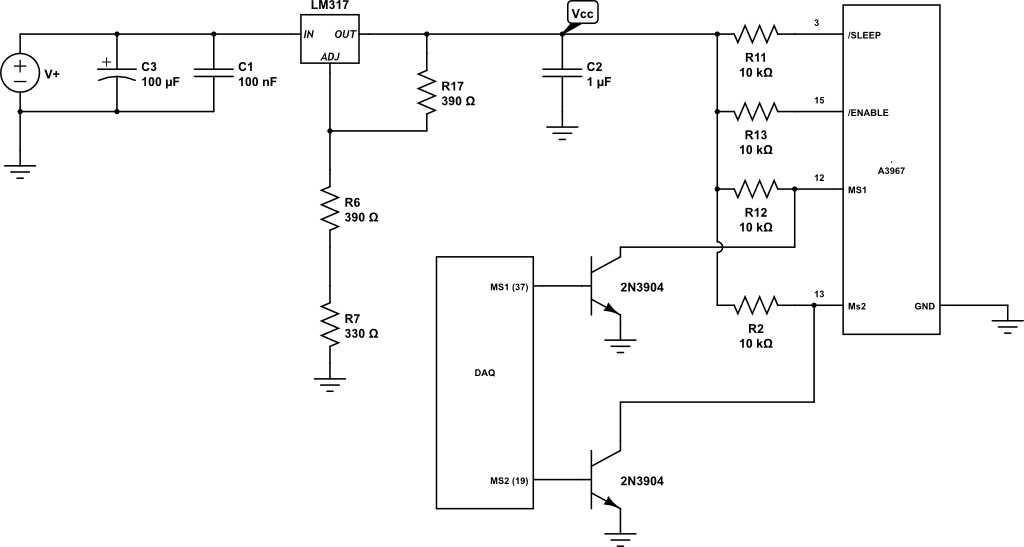
\includegraphics[width = 18cm]{lab5_q1_c.png}
\caption{Ideal Sleep, Enable, MS1 and MS2 pins connection diagram. \emph{Note all grounds are common}}
\label{q1_c}
\end{center}
\end{figure}

Figure \ref{q1_c} shows the ideal connection diagrams for the EasyDriver pcb along with some of the default connections already made on the board. The Sleep and Enable pins are low-enable pins. As we do not explicitly need to control them, we leave them in their default connection - with the EasyDriver pulling them up to $V_{cc}$.\\

$V_{cc}$is generated through passing the main supply voltage through an LM317 voltage regulator that provides a relatively clean and stable 5V \footnote{Or 3.3V depending on the settings.}. This $V_{cc}$ is then used by the EasyDriver circuit to pull up pins as required. We use a 10$k\Omega$ resistor in series with the pin to act as a buffer resistor and so that if an external circuit is used to ground the pin, $V_{cc}$ is not connected to the ground directly.\\

For MS1 and MS2, we wish to control their states. By default the EasyDriver circuit pulls MS1 and MS2 upto $V_{cc}$.Ideally to pull them to the ground potential we should use a decoupling transistor circuit as shown in figure \ref{q1_c}. This would then require the MS1 and MS2 control logic to be inverted as a high output would power the transistors to bring the pin potential to the ground. This design would electrically isolate the DAQ from the circuits.\\

 However, in our actual implementation, we connected the pin directly to the DAQ. This works as we have high quality DAQ that can handle small circulating currents if they do arise\footnote{Due to mismatches in voltages.}.\\

The only change from defaults we incorporated was connecting MS1 and MS2. this was done to control the step size. 


\subsection*{d.}
We provided the 5V supply to our optical encoder from our external power source, the T60c switching power supply. Doing so has the following advantage:
\begin{itemize}
\item It provides a cleaner 5V - The circuitry on board the main power supply has more sophisticated circuitry than the LM741 regulator.

\item It has better cooling - The T60c is designed for high power output and as such is equipped for cooling.

\item Loading effects of the motor are not seen - if the motor draws a lot of power, its effects would be seen across the output of the voltage regulator. By decoupling the encoder power source from the motor driver, we can provide power irrespective of the power demands of the motor.
\end{itemize}

However it does also have the following disadvantages:
\begin{itemize}
\item 5V source could be contaminated with 60Hz noise - the T60 takes in 60Hz AC supply which could cause electromagnetic interference in the 5V supply.

\item The system becomes more spread out - using the 5V supply of the EasyDriver provides a more compact solution which helps us treat the system like a black box. Choosing the T60c would mean more wires come out of the system and hence more cabling costs.

\end{itemize}

Given the advantages and disadvantages, we chose the more reliable choice as we are only building a stationary prototype. Hence we can ignore any space constraints.


\section{LabView Implementation}
Figures \ref{q2_1} and \ref{q2_2} show the front panel and block diagram, respectively, of the LabView VI created to meet the requirements in the Lab 5 Instructions, as well as additional inputs and outputs for debugging. The front panel includes inputs for the user to select the mode (velocity vs. position), direction of rotation, step size, and input value with options for type of units (ie. position as number of degrees or number of steps). Additionally, there is an overall power button (labeled "GO") and an option to save the encoder data using the "Write to Measurement File" block. In practice this option was rarely used as it tended to slow down the simulation loop when set to high frequencies (over about 200 Hz).\\

The main output on the front panel is the "Motor Angle" waveform chart which displays the angular displacement obtained from the encoder via quadrature decoding. There is also a waveform chart for angular velocity which is only used for steady-state estimations for debugging as the filter used creates a significant delay. More accurate velocity values were obtained by exporting the displacement data and fitting lines to calculate slope. Additional debugging outputs consist of the "sum" indicator (which displays the current value of the edge counter), and LEDs for each of the outputs to the motor driver.     \\


\begin{figure}[hbt]
\begin{center}
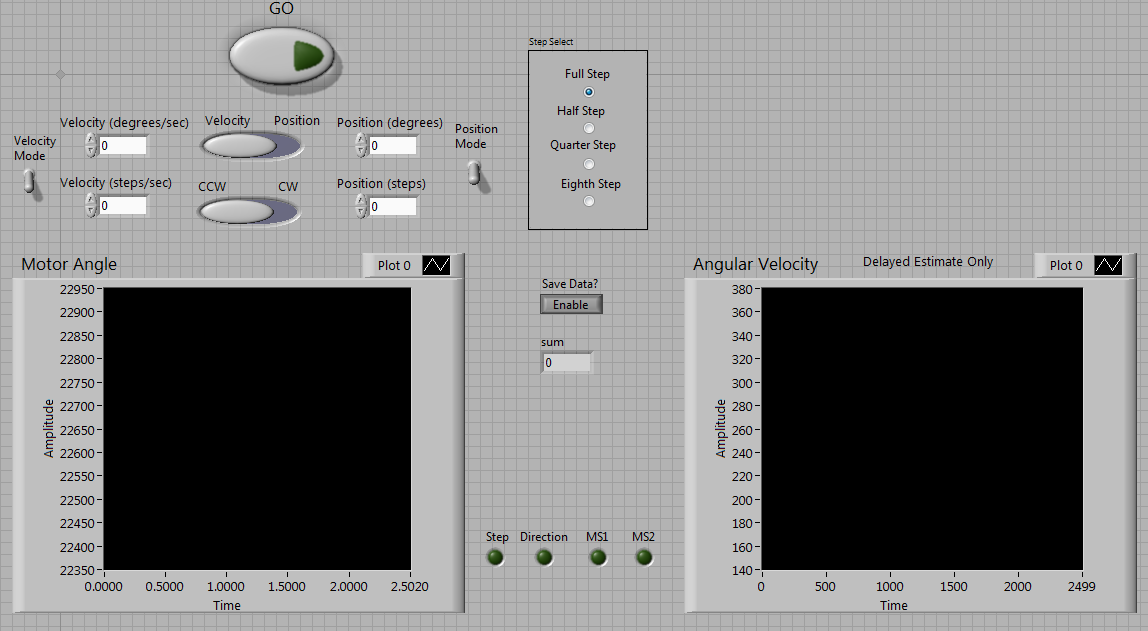
\includegraphics[width = 18cm]{VIFrontPanel.png}
\caption{Front panel of primary LabView VI.}
\label{q2_1}
\end{center}
\end{figure}

\begin{figure}[hbt]
\begin{center}
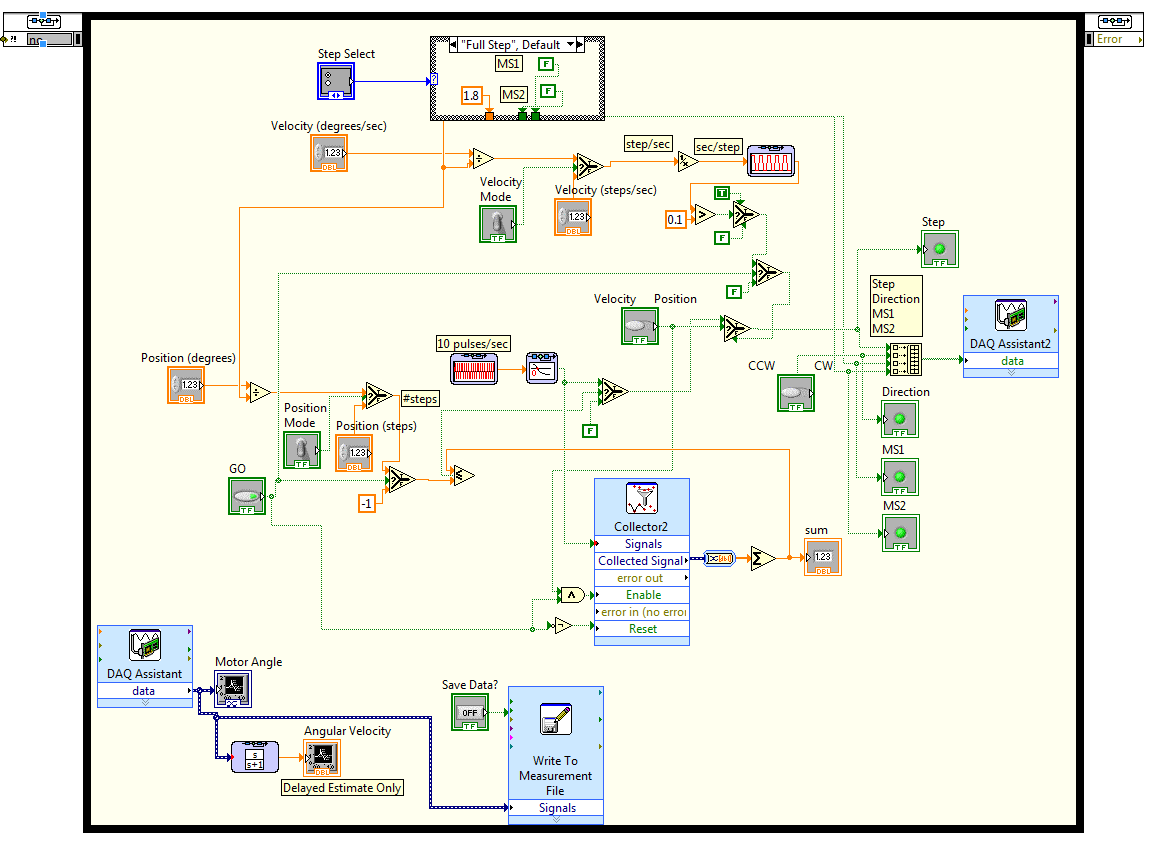
\includegraphics[width = 18cm]{VIBlockDiagram.png}
\caption{Block diagram of primary LabView VI.}
\label{q2_2}
\end{center}
\end{figure}

The VI uses a control \& simulation loop running at 1000 Hz. At the top of the block diagram in figure \ref{q2_2} is a radio button block connected to a case structure. This is the step size selector. Depending on the button selected by the user, a constant is output corresponding to the degrees per step for that step size, and booleans are output for MS1 and MS2 according to the settings given in table \ref{q1_b3}.\\

Below the case structure is the velocity control segment of the VI. Based on the users desired velocity, unit type, and step size, the number of steps per second is calculated and used to set the period of a "Pulse Signal" block. A greater than comparator is then used to convert the 1's and 0's of the pulse signal into a stream of true and false booleans. This stream is put into an array along with a boolean for the direction of rotation and booleans for MS1 and MS2. This array is then sent to a DAQ Assistant block, which sends the array elements to the motor driver. Smaller step sizes resulted in smoother operation, but were not achievable at high velocities. Therefore, we left the step size as selectable rather than setting a specific step size.\\

In the middle of the block diagram is the position control section. At all times, a pulse generator is running at 10 Hz (arbitrarily selected; this could be a user input). The pulse signal is shifted downwards so that a zero crossing block can be used to detect the rising edges of the signal. Every time a rising edge is detected, the zero crossing block sends out a true boolean. However, this value only reaches the output array if the user has selected position mode and has selected the GO button. To stop after the desired number of steps has been taken, the output of the zero crossing block is also sent to a "Collector" block, which stores the values like an array. Summing the values within the collector gives the number of steps that have been taken. However, the collector is only enabled when the user selects position mode and the GO button (this makes the VI run faster in velocity mode, allowing for higher velocities). Additionally, the collector continuously resets itself when GO is not selected. This allows for multiple runs, and prevents the always running pulse signal from storing edge counts when not desired. The user's desired displacement is converted to the number of steps required, and a less-than-or-equal-to comparator is used to stop the stream of pulses to the output when the edge count reaches the required number of steps.\\

At the bottom of the block diagram is the input from the encoder, which is not used for control feedback. A derivative and filter are used to display the angular velocity. However, there is a significant delay, to the velocity chart was only used for debugging at steady-state. A block to save the encoder data to a file is provided, but was rarely used as it had a significant negative impact on the speed of the simulation loop.   \\

\clearpage

\section{Experimental Characterization}
\subsection*{a.}
\subsubsection*{i}
\subsubsection*{ii}
\subsection*{b.}

\clearpage

\section{Motion Control}
\subsection*{a.}
\subsection*{b.}
\subsection*{c.}

\clearpage




\clearpage
\section*{Appendix.}

\subsection*{System Energy Computation}
\xxx{Uncomment below to add m-file code}
%\verbatiminput{totalEnergy.m}

\end{document}